\documentclass[aspectratio=169,11pt]{beamer}

\usepackage[utf8]{inputenc}
\usepackage[T1]{fontenc}
\usepackage[brazil]{babel}
\usepackage{lmodern}
\usepackage{amsmath,amssymb}
\usepackage{booktabs}
\usepackage{graphicx}
\usepackage{tikz}
\usetikzlibrary{positioning}

% ── Tema ──────────────────────────────────────────────────────────────────────
\usetheme{Madrid}
\usecolortheme{whale}
\setbeamercolor{frametitle}{bg=structure.fg!82!black, fg=white}
\setbeamercolor{block title}{bg=structure.fg!70!black, fg=white}
\setbeamercolor{alerted text}{fg=orange!85!black}
\setbeamerfont{frametitle}{size=\large,series=\bfseries}
\setbeamertemplate{navigation symbols}{}

% Rodap\'{e}: altura fixa 4ex para n\~{a}o cortar nomes
\setbeamertemplate{footline}{%
  \leavevmode%
  \hbox{%
    \begin{beamercolorbox}[wd=.50\paperwidth,ht=4ex,dp=1.5ex,center]{author in head/foot}%
      \usebeamerfont{author in head/foot}%
      Leandro \textperiodcentered{} Leon \textperiodcentered{} Vithoria%
    \end{beamercolorbox}%
    \begin{beamercolorbox}[wd=.35\paperwidth,ht=4ex,dp=1.5ex,center]{title in head/foot}%
      \usebeamerfont{title in head/foot}T\'{o}picos em Otimiza\c{c}\~{a}o -- UFRPE%
    \end{beamercolorbox}%
    \begin{beamercolorbox}[wd=.15\paperwidth,ht=4ex,dp=1.5ex,right]{date in head/foot}%
      \usebeamerfont{date in head/foot}%
      \insertframenumber/\inserttotalframenumber\hspace*{2ex}%
    \end{beamercolorbox}%
  }%
}

% Margem extra no conte\'{u}do para n\~{a}o encostar no rodap\'{e}
\setbeamersize{text margin left=6mm, text margin right=6mm}
\addtobeamertemplate{frametitle}{}{\vspace{-1mm}}

% ── Metadados ─────────────────────────────────────────────────────────────────
\title[Atribui\c{c}\~{a}o de Leads -- BFC]{%
  Problema de Atribui\c{c}\~{a}o de Leads Comerciais\\
  em uma Startup de Impacto}
\subtitle{Uma Abordagem de Otimiza\c{c}\~{a}o Combinat\'{o}ria\\
  para Maximiza\c{c}\~{a}o de Retorno}
\author[Leandro \textperiodcentered{} Leon \textperiodcentered{} Vithoria]{%
  Leandro Dos Santos Cesar \and
  Leon Louren\c{c}o da Silva Santos \and
  Vithoria Camila Bastos da Silva}
\institute{Universidade Federal Rural de Pernambuco\\T\'{o}picos em Otimiza\c{c}\~{a}o}
\date{Junho de 2026}

% ── Cores ─────────────────────────────────────────────────────────────────────
\definecolor{Cazul}{RGB}{44,95,138}
\definecolor{Cclaro}{RGB}{168,200,232}
\definecolor{Ccinza}{RGB}{140,140,140}
\definecolor{Cverde}{RGB}{30,132,73}

% ── Comando auxiliar: n\'{u}mero grande com r\'{o}tulo abaixo ─────────────────────────
\newcommand{\bigstat}[2]{%
  \begin{center}
    {\fontsize{36}{40}\selectfont\bfseries\color{Cazul}#1}\\[2pt]
    {\small\color{Ccinza}#2}
  \end{center}%
}

% =============================================================================
\begin{document}

% ── 1. Capa ───────────────────────────────────────────────────────────────────
\begin{frame}
  \titlepage
\end{frame}

% =============================================================================
\section{O Problema}
% =============================================================================

% ── 2. Contexto visual ────────────────────────────────────────────────────────
\begin{frame}{A Biof\'{a}brica de Corais e o desafio comercial}
\begin{columns}[c]

\begin{column}{0.38\textwidth}
  \textbf{Biof\'{a}brica de Corais (BFC)}\\[0.5em]
  \small Startup pernambucana de restaura\c{c}\~{a}o de recifes
  e educa\c{c}\~{a}o ambiental. Produtos que v\~{a}o de associa\c{c}\~{o}es
  individuais a projetos PDI/ESG corporativos.

  \vspace{0.8em}
  \bigstat{113}{leads no CRM}
  \bigstat{37}{leads ativos}
  \bigstat{3}{vendedores}
\end{column}

\begin{column}{0.02\textwidth}
  \textcolor{Cclaro}{\rule{0.8pt}{0.68\textheight}}
\end{column}

\begin{column}{0.57\textwidth}
  \begin{center}
  \begin{tikzpicture}[
      lead/.style={draw=Cazul, fill=Cclaro, rounded corners=3pt,
                   minimum width=2.8cm, minimum height=0.55cm,
                   align=center, font=\scriptsize},
      vend/.style={draw=Cazul!80!black, fill=Cazul, text=white,
                   rounded corners=3pt,
                   minimum width=2.6cm, minimum height=0.55cm,
                   align=center, font=\scriptsize},
      scale=0.92]
    % Leads
    \node[lead] (L1) at (0, 2.2)  {Simone \tiny(PJ, Alto)\\$w =$ R\$\,7.800};
    \node[lead] (L2) at (0, 1.1)  {Monica \tiny(PF, Alto)\\$w =$ R\$\,1.625};
    \node[lead] (L3) at (0, 0.0)  {Ana B\'{a}rbara \tiny(PJ)\\$w =$ R\$\,679};
    \node[lead] (L4) at (0,-1.1)  {Lucas Diniz \tiny(PJ)\\$w =$ R\$\,659};
    \node[lead] (L5) at (0,-2.2)  {Marina Barck\\$w =$ R\$\,191};
    % Vendedores
    \node[vend] (V1) at (5.2, 1.4)  {Marcela Belo};
    \node[vend] (V2) at (5.2, 0.0)  {Maria Paula};
    \node[vend] (V3) at (5.2,-1.4)  {Talita Guedes};
    % Arestas (espessura prop. a w)
    \draw[Cazul, line width=3.2pt, opacity=0.75] (L1.east) -- (V1.west);
    \draw[Cazul, line width=1.3pt, opacity=0.55] (L2.east) -- (V1.west);
    \draw[Cazul, line width=1.3pt, opacity=0.55] (L2.east) -- (V2.west);
    \draw[Cazul, line width=0.7pt, opacity=0.45] (L3.east) -- (V2.west);
    \draw[Cazul, line width=0.7pt, opacity=0.45] (L4.east) -- (V3.west);
    \draw[Cazul, line width=0.3pt, opacity=0.35] (L5.east) -- (V3.west);
    % R\'{o}tulos
    \node[font=\small\bfseries, color=Cazul] at (0, 3.0)   {Leads ($L$)};
    \node[font=\small\bfseries, color=Cazul] at (5.2, 3.0) {Vendedores ($V$)};
    % Legenda
    \node[font=\tiny, color=Ccinza] at (2.6,-3.0)
      {espessura da aresta $\propto$ valor esperado $w_{ij}$};
  \end{tikzpicture}
  \end{center}
\end{column}

\end{columns}
\end{frame}

% ── 3. A quest\~{a}o central ───────────────────────────────────────────────────────
\begin{frame}{A quest\~{a}o}
\vspace{0.8em}
\begin{center}
  {\Large\textit{``Como alocar o tempo da equipe comercial\\[0.4em]
  sobre os leads dispon\'{i}veis de forma a\\[0.4em]
  \alert{maximizar a receita esperada total?}''}}
\end{center}
\vspace{1.4em}
\begin{center}
\begin{tikzpicture}
  \node[draw=Cazul, fill=Cclaro, rounded corners=5pt,
        minimum width=5cm, minimum height=1.2cm,
        font=\normalsize, align=center]
    (A) {Sem crit\'{e}rio formal:\\leads atendidos por intui\c{c}\~{a}o};
  \node[draw=Cverde, fill=Cverde!15, rounded corners=5pt,
        minimum width=5cm, minimum height=1.2cm,
        font=\normalsize, align=center, right=1.5cm of A]
    (B) {Com otimiza\c{c}\~{a}o:\\aloca\c{c}\~{a}o por valor esperado};
  \draw[->, thick, Cazul] (A.east) -- (B.west);
\end{tikzpicture}
\end{center}
\end{frame}

% =============================================================================
\section{Modelagem}
% =============================================================================

% ── 4. O modelo ───────────────────────────────────────────────────────────────
\begin{frame}{O modelo: valor esperado de cada lead}
\begin{columns}[c]

\begin{column}{0.48\textwidth}
  \begin{center}
    \vspace{0.6em}
    {\Large $w_i \;=\; p_c \;\times\; V_t$}\\[1.0em]
    \small
    \begin{tabular}{cl}
      $p_c$ & probabilidade de convers\~{a}o \\[2pt]
      $V_t$ & valor estimado do contrato \\
    \end{tabular}
  \end{center}

  \vspace{1.2em}
  \begin{center}
    \begin{tabular}{lc}
      \toprule
      Interesse declarado & $p_c$ \\
      \midrule
      Muito Alto & 0,85 \\
      Alto       & 0,65 \\
      Moderado   & 0,55 \\
      M\'{e}dio  & 0,45 \\
      Baixo      & 0,20 \\
      Sem dado   & 0,10 \\
      \bottomrule
    \end{tabular}
  \end{center}
\end{column}

\begin{column}{0.48\textwidth}
  \vspace{0.4em}
  \textbf{Dois enquadramentos cl\'{a}ssicos:}

  \vspace{0.8em}
  \begin{block}{Mochila Bin\'{a}ria}
    \centering
    $\max \displaystyle\sum w_i \;\;\text{s.a.}\;\; \sum t_i \leq C$\\[2pt]
    \small Quais leads atender?
  \end{block}

  \vspace{0.6em}
  \begin{alertblock}{Matching Bipartido}
    \centering
    $\max \displaystyle\sum_{(l_i,v_j)} w(l_i,v_j)$\\[2pt]
    \small Quem atende quem? (respeita cota por vendedor)
  \end{alertblock}
\end{column}

\end{columns}
\end{frame}

% =============================================================================
\section{Dados e Resultados}
% =============================================================================

% ── 5. Carteira ativa ─────────────────────────────────────────────────────────
\begin{frame}{Carteira ativa: distribui\c{c}\~{a}o de valor}
  \begin{center}
    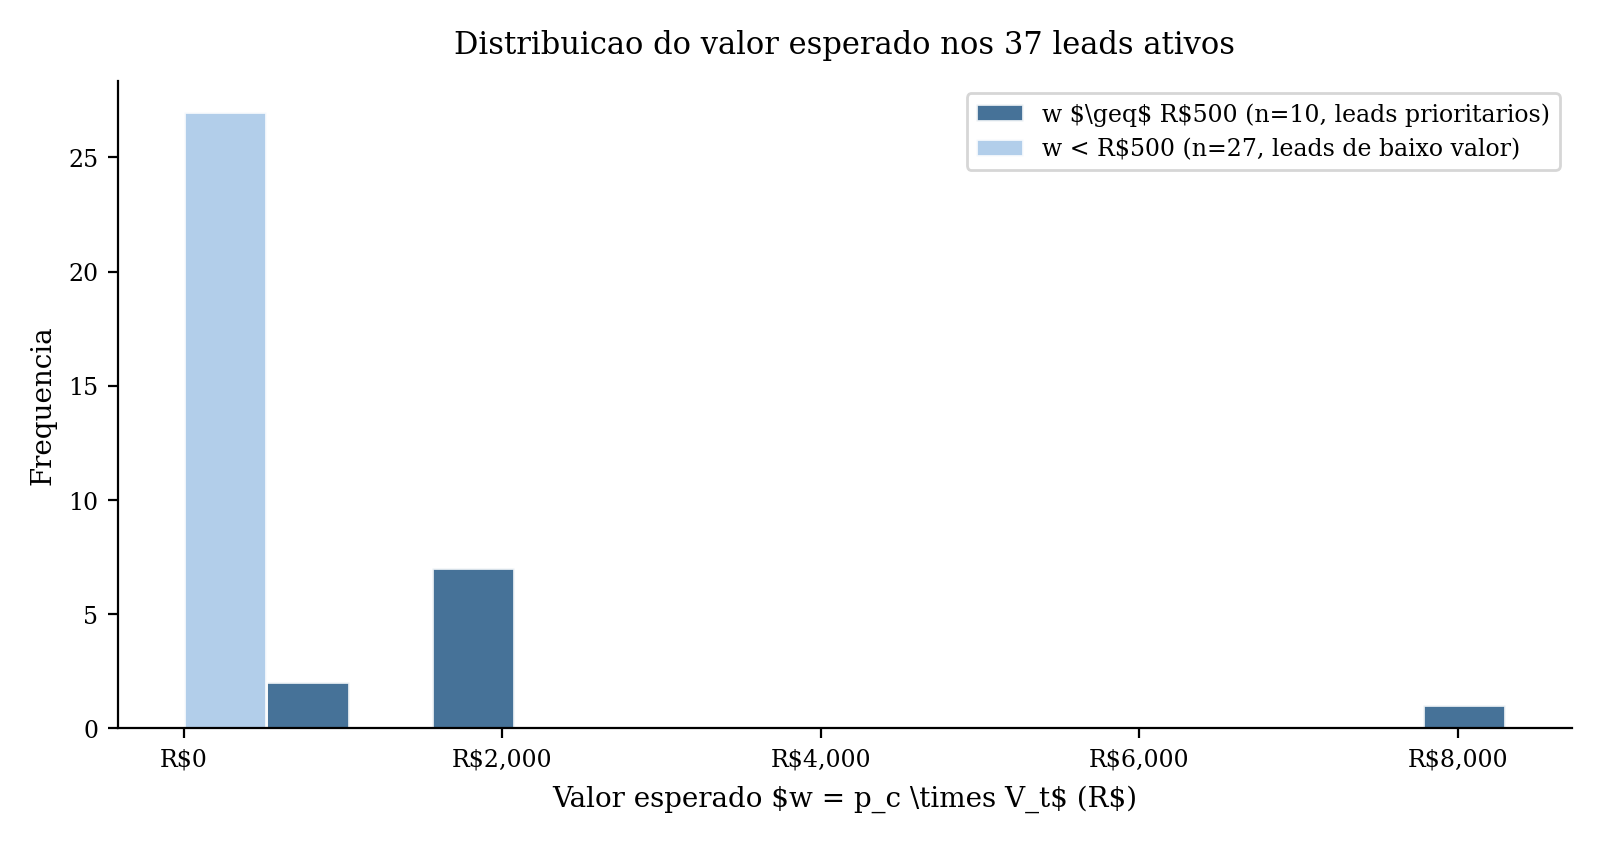
\includegraphics[width=0.82\textwidth, height=0.72\textheight,
                     keepaspectratio]{art_fig6_dist_valor.png}
  \end{center}
\end{frame}

% ── 6. Achado estrutural ──────────────────────────────────────────────────────
\begin{frame}{O achado que muda a pergunta}
\begin{columns}[c]

\begin{column}{0.45\textwidth}
  \begin{center}
    \begin{tikzpicture}[scale=1.0]
      % Trilho cinza (100 h)
      \fill[Cclaro!50] (0,0) rectangle (5,0.9);
      \draw[Ccinza!70, thin] (0,0) rectangle (5,0.9);
      % Preenchimento azul (72,5 h = 72.5%)
      \fill[Cazul] (0,0) rectangle (3.625,0.9);
      % Valor dentro da barra azul
      \node[white, font=\bfseries\normalsize] at (1.81,0.45) {72,5 h};
      % Valor fora (parte clara) -- acima para nao colidir
      \node[Ccinza!80!black, font=\small\bfseries] at (4.31,0.45) {27,5 h};
      % R\'{o}tulos separados abaixo
      \node[font=\scriptsize, Cazul, anchor=west] at (0,-0.38)
        {Tempo para 37 leads};
      \node[font=\scriptsize, Ccinza, anchor=east] at (5,-0.38)
        {Total dispon\'{i}vel: 100 h};
    \end{tikzpicture}

    \vspace{1.6em}
    {\LARGE\bfseries\alert{72,5 h $<$ 100 h}}
  \end{center}
\end{column}

\begin{column}{0.50\textwidth}
  \vspace{0.5em}
  \begin{block}{}
    \centering
    A pergunta n\~{a}o \'{e} mais\\[0.3em]
    \textit{``quais leads descartar?''}\\[0.7em]
    e passa a ser\\[0.7em]
    \textbf{``como distribuir os leads\\
    entre os vendedores?''}
  \end{block}
\end{column}

\end{columns}
\end{frame}

% ── 7. Comparativo ────────────────────────────────────────────────────────────
\begin{frame}{Comparativo dos tr\^{e}s algoritmos}
  \begin{center}
    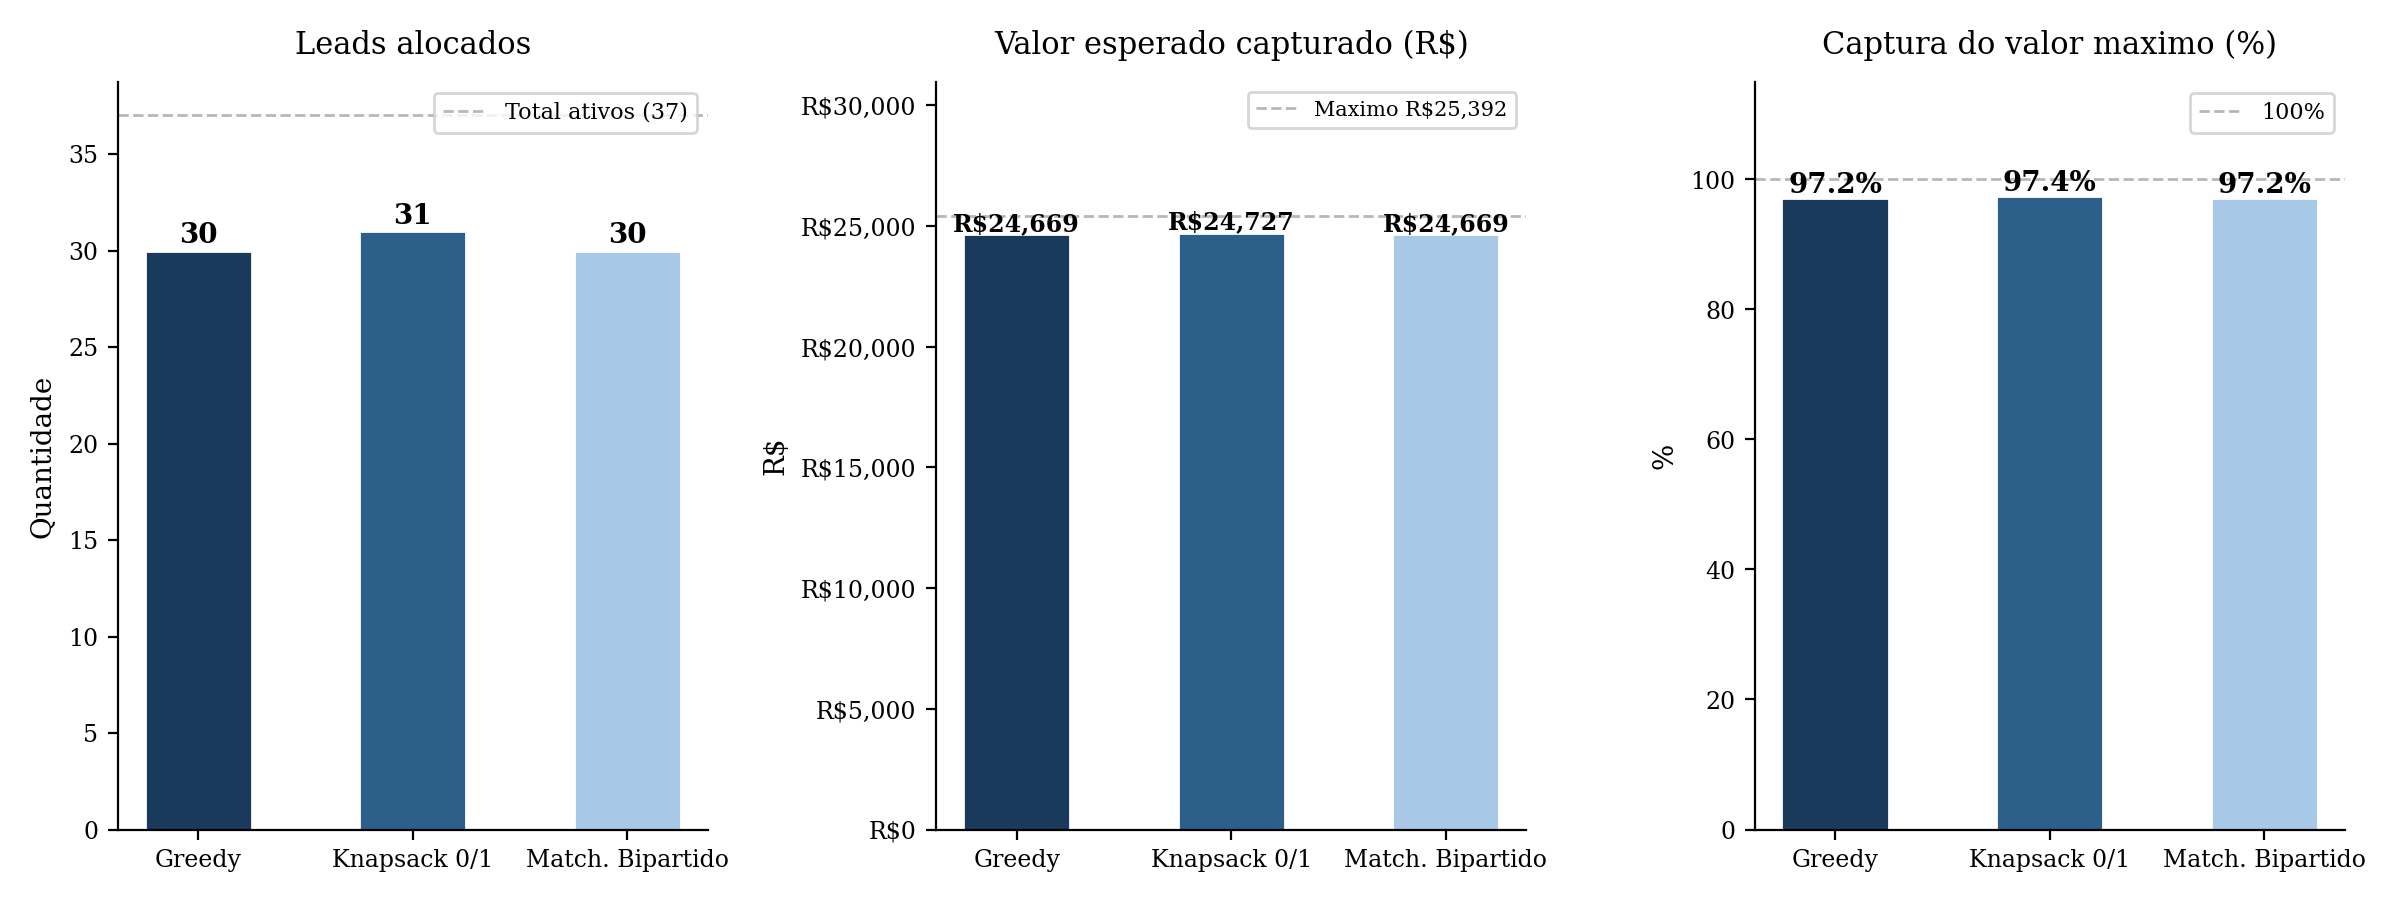
\includegraphics[width=\textwidth, height=0.74\textheight,
                     keepaspectratio]{art_fig5_comparacao.png}
  \end{center}
\end{frame}

% ── 8. Distribui\c{c}\~{a}o Matching ──────────────────────────────────────────────────
\begin{frame}{Matching Bipartido: carga por vendedor}
  \begin{center}
    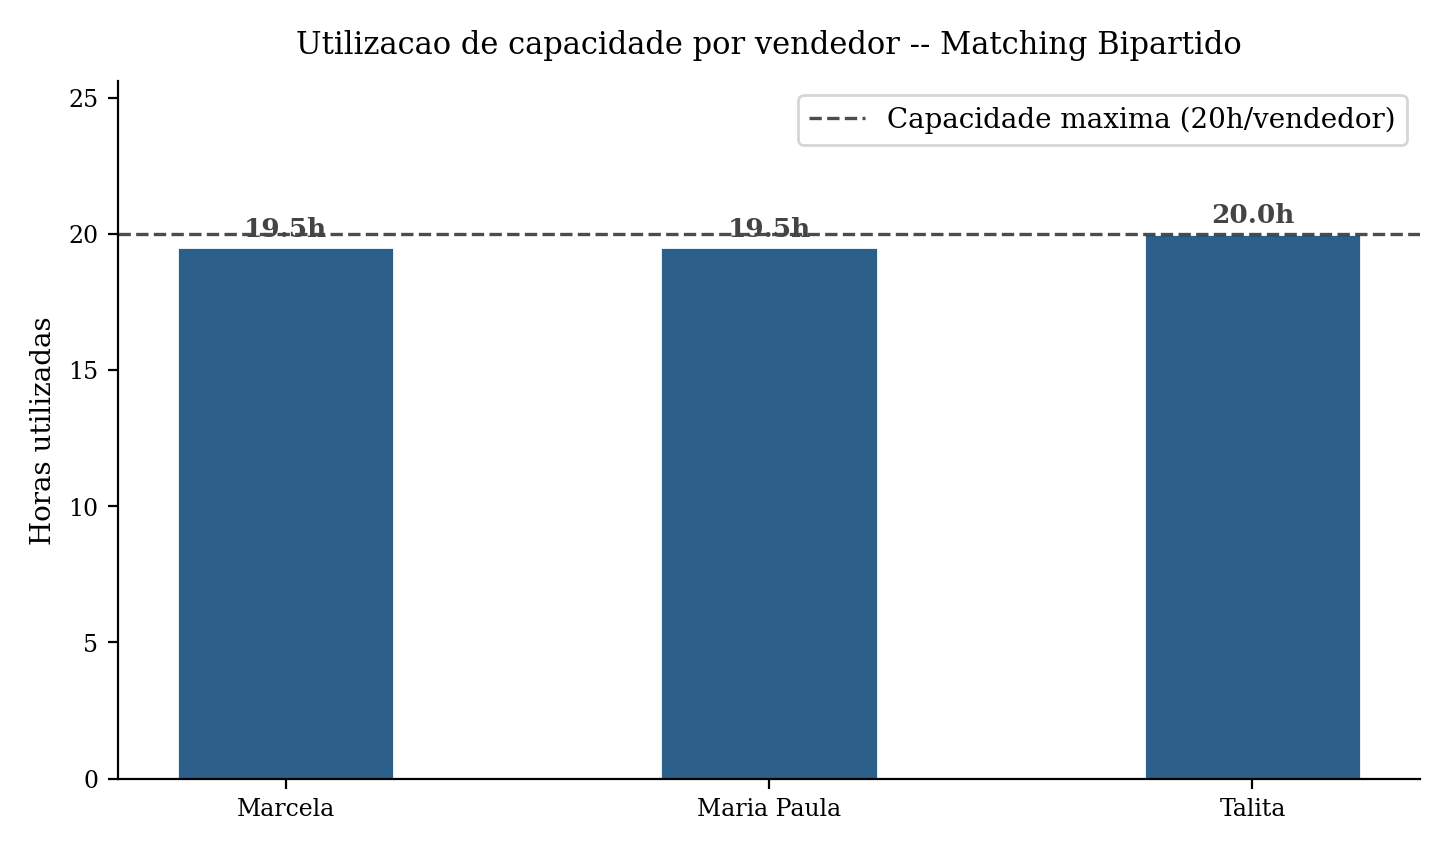
\includegraphics[width=0.80\textwidth, height=0.74\textheight,
                     keepaspectratio]{art_fig7_cap_vendedor.png}
  \end{center}
\end{frame}

% =============================================================================
\section{Conclus\~{a}o}
% =============================================================================

% ── 9. Resposta ───────────────────────────────────────────────────────────────
\begin{frame}{Resposta \`{a} quest\~{a}o central}
\vspace{0.4em}
\begin{columns}[T]

\begin{column}{0.48\textwidth}
  \begin{block}{Todos os leads cabem}
    \small 72,5 h $<$ 100 h dispon\'{i}veis.\\
    Atender todos os 37 leads neste ciclo.
  \end{block}

  \vspace{0.7em}
  \begin{block}{Prioriza\c{c}\~{a}o}
    \small 8 leads concentram 85,5\% do valor.\\
    Esses v\~{a}o para os melhores vendedores.
  \end{block}
\end{column}

\begin{column}{0.48\textwidth}
  \begin{block}{Trade-off de distribui\c{c}\~{a}o}
    \small
    \textbf{Greedy / Knapsack:} 100\% do valor capturado.\\[4pt]
    \textbf{Matching:} equidade de carga entre vendedores,
    com perda de \alert{$\approx$10\%} do valor esperado.
  \end{block}
\end{column}

\end{columns}
\end{frame}

% ── 10. Conclus\~{a}o ─────────────────────────────────────────────────────────────
\begin{frame}{Conclus\~{a}o}
\begin{columns}[T]

\begin{column}{0.48\textwidth}
  \textbf{O que foi feito}
  \vspace{0.3em}
  \begin{itemize}\setlength\itemsep{4pt}
    \item 113 leads reais modelados como grafo e mochila
    \item 3 algoritmos implementados e comparados
    \item Resposta quantitativa \`{a} quest\~{a}o de aloca\c{c}\~{a}o
  \end{itemize}
\end{column}

\begin{column}{0.48\textwidth}
  \textbf{Limita\c{c}\~{o}es}
  \vspace{0.3em}
  \begin{itemize}\setlength\itemsep{4pt}
    \item 99\% dos valores de contrato s\~{a}o estimativas
    \item 41\% dos leads sem interesse declarado
    \item Afinidade vendedor-lead n\~{a}o calculada
  \end{itemize}
\end{column}

\end{columns}

\vspace{1.2em}
\begin{center}
  \large\textit{A otimiza\c{c}\~{a}o come\c{c}a pelo CRM.}
\end{center}
\end{frame}

% ── 11. Encerramento ──────────────────────────────────────────────────────────
\begin{frame}[plain]
  \vspace{2.5em}
  \begin{center}
    {\LARGE\bfseries Obrigado!}\\[1.4em]
    Leandro Dos Santos Cesar\\
    Leon Louren\c{c}o da Silva Santos\\
    Vithoria Camila Bastos da Silva\\[1.4em]
    \textit{T\'{o}picos em Otimiza\c{c}\~{a}o -- UFRPE, Junho de 2026}
  \end{center}
\end{frame}

\end{document}
